\section{Introduction}

The James Webb Space Telescope (JWST) will offer an early chance to characterize small worlds, through measurements of their bulk densities, and transmission spectroscopy of their atmospheres. The integration times required to produce transmission spectra will be highly expensive, so it's likely that only a handful of small planets will be observed in transmission by JWST with sufficient signal-to-noise to characterize there atmospheres and densities \citep{Cowan2015}.

We can measure densities of some transiting worlds in multiplanet systems with transit timing variations (TTVs) \citep{Agol2005, Holman2005}. This technique allows us to measure the masses of planets in multi-planet systems by via their gravitational influence on each other, causing some transits to appear earlier than expected, and others later. The  variations in transit times are related to the masses and eccentricities of each planet, enabling us to measure exoplanet masses, relative to their star, with photometry alone. TTVs are especially promising for measuring the masses of small, potentially habitable worlds which are too small and far from their stars to impart measurable radial velocities on their host stars. Recent work by \citet{Deck2014, Agol2016a, Agol2016b} makes forward-modeling of TTVs computationally efficient enough to sample for planet masses and eccentricities with Monte Carlo techniques. 

We can measure the atmospheric compositions of exoplanets with transmission spectroscopy. At wavelengths where an exoplanet's atmosphere is opaque, the planet will appear larger in transit than at wavelengths where the atmosphere is transparent, allowing us to measure an absorption spectrum of the planet's atmosphere from measurements of the wavelength-dependent transit depth. JWST will be the first telescope capable of measuring transmission spectra of small, rocky exoplanet atmospheres. Fortuitously, transit timing measurements can be derived from any transit observations, including transmission spectroscopy, for example.

In this work, we focus on the potential for characterization of three pairs of planets: TRAPPIST-1 b and c, Kepler-62 e and f, and Kepler-296 e and f. TRAPPIST-1 is an M8 dwarf with at least three habitable, Earth-sized planets \citep{Gillon2016, Gillon2017, Delrez2018}. Kepler-62 is a K2 dwarf with $\sim$one habitable, Earth-sized planet \citep{Borucki2013}, and Kepler-296 is an M1 star with five planets and an M4 companion \citep{Barclay2015}.

Stellar atmospheres introduce a variety of challenges to transit characterization \citep{Rackham2018, Zhang2018}. Rotational variability due to starspots and  ``microvariability''  as observed on TRAPPIST-1 by \citet{Delrez2018} are sources of astrophysical noise with amplitudes greater than or similar to the photon-noise on each target. Any analysis of the transit times and transmission spectra of the planets of these stars must account for the time- and wavelength-dependent variability of heterogeneous stellar atmospheres.

\section{Targets}

\begin{figure}
\centering
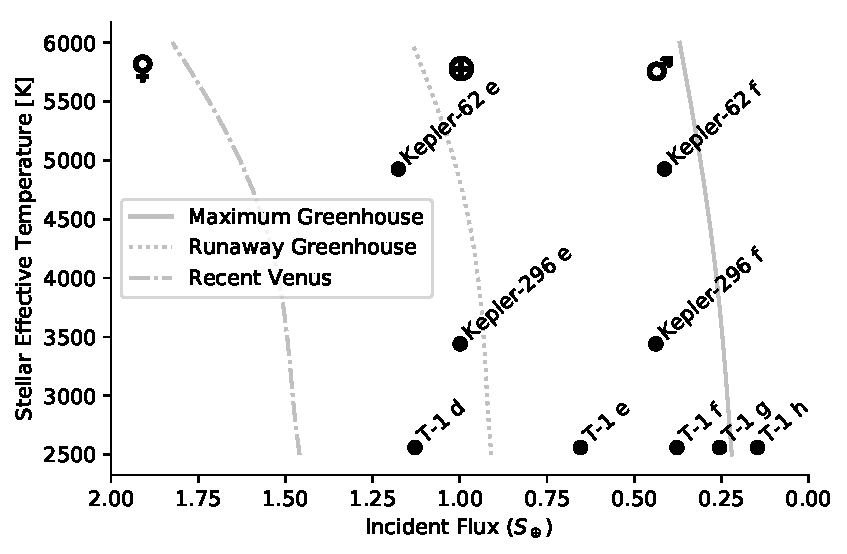
\includegraphics[scale=0.58]{libra/census.pdf}
\caption{Habitable zone planets under consideration for mass measurements with TTVs from JWST \citep{Borucki2013, Delrez2018}. We also mark the limits of the habitable zone defined by \citet{Kopparapu2013}.}
\label{fig:census}
\end{figure}

\subsection{TRAPPIST-1}

TRAPPIST-1 is a M8V host to seven small planets in a resonant chain \citep{Gillon2016, Gillon2017, Luger2017, Delrez2018}. Dynamical simulations show that most of the planets are consistent with Earth-like masses \citep{Quarles2017}. The habitability of the worlds in the TRAPPIST-1 system is up for debate -- the inner planets suffer from dessication when the star is young and hot \citep{Luger2015, Bolmont2017}. The star is active, and its flares and UV activity may be hazardous to life on the planets \citep{Vida2017, Davenport2017, Roettenbacher2017}. 

Characterization of the rotation period and stellar activity of TRAPPIST-1 has proven beguiling \citep{Roettenbacher2017, Morris2018c, Rackham2018, Zhang2018}, though its age is well constrained ($7.6 \pm 2.2$ Gyr) \citep{Burgasser2017}. 

% Planet-planet occultations \citep{Luger2017b}. 

\subsection{Kepler-296}

Kepler-296 is a M1V host to five transiting planets, and it is also orbited by a M4V companion \citep{Lissauer2014, Torres2015, Barclay2015}. 

\subsection{Kepler-62}

Kepler-62 is a K2V host to five transiting planets \citep{Borucki2013}. Planets e and f are potentially habitable. \citet{Kaltenegger2013} proposed these could be water planets. \citet{Shields2016} ran global climate models to show what atmospheric chemistry and orbital dynamics are necessary to maintain habitability for planet f. Tides are important to consider for habitability \citep{Bolmont2014, Bolmont2015}.

Unlike the TRAPPIST-1 planets, Kepler-62 f is far enough from its host to avoid desiccation in the hot, pre-main sequence phase, and could retain liquid water \citep{Luger2015}. 

% \subsection{Photon-noise limited analysis}

% We select two candidates for JWST observations by considering a photon-noise limited transit observation for each planet in each system. We generate simulated transit observations using NIRSpec with the Prism/Clear mode without simulating starspots, flares, granulation or instrumental systematics. Then we fit the simulated light curve with MCMC to solve for the posterior uncertainty on the mid-transit times to find the best-case mid-transit time uncertainty. 

% \begin{table}
% \begin{center}
% \begin{tabular}{lcc}
% Planet & $\sigma_T$  & $\sigma_M$ \\
%  & [s] & [$M_{\oplus}$] \\\hline\hline
% Kepler-296 b & 14.576 & \\
% Kepler-296 c & 8.190 & \\
% Kepler-296 d & 9.952 & \\
% Kepler-296 e & 19.842 & \\
% Kepler-296 f & 15.638 & \\ \hline
% TRAPPIST-1 b & 0.588 & \\
% TRAPPIST-1 c & 2.855 & \\
% TRAPPIST-1 d & 0.953 & \\
% TRAPPIST-1 e & 0.974 & \\
% TRAPPIST-1 f & 0.948 & \\
% TRAPPIST-1 g & 2.021 & \\
% TRAPPIST-1 h & 1.575 & \\
% \end{tabular}
% \end{center}
% \caption{Posterior midtransit time uncertainties for candidate TTV planets, assuming the observations are only photon-limited, with one second exposures for TRAPPIST-1, and 100 second exposures for the dimmer stars Kepler-296 and Kepler-62. This best-case analysis shows that observations of the TRAPPIST-1 planets will yield mass constraints more efficiently than similar systems.  \label{tab:photon_limited}}
% \end{table}


\section{Simulated Observations}

\subsection{JWST Observing Mode: NIRSpec/Prism BOTS}

JWST's NIRSpec infrared spectrograph has a Bright Object Time Series (BOTS) observing mode, with the 1.6 $\times$ 1.6" S1600A1 aperture and the prism/clear filter to collect spectra with resolution $R\sim100$. The SUB512 subarray yields spectra with 512 $\times$ 32 pixels. The frame time, or the duration of an individual sample up-the-ramp, is 0.226 s. 

Even with this short frame time, some pixels will be saturated by TRAPPIST-1 (J=11.354) for $N_\mathrm{group} > 2$, where $N_\mathrm{group}$ is the number of frames per ``group''. However, we should be able to measure the flux in those pixels with first 2-3 samples up-the-ramp of each group \citep[see also][]{Batalha2018}. We therefore choose to simulate observations of TRAPPIST-1 with $N_\mathrm{group} = 6$, which saturates $<1\%$ of pixels, centered near 1.75 $\mu$m. This observing strategy yields the on-sky observing efficiency 71.4\%. 

For the slightly dimmer Kepler-62 (J=12.256), we also choose to observe with $N_\mathrm{group} = 6$, which is dim enough to avoid saturation. For the significantly dimmer Kepler-296 (J=13.391), we can manage to osberve $N_\mathrm{group} = 18$ without saturating the detector for observing efficiency of 90\%.

\begin{figure}
    \centering
    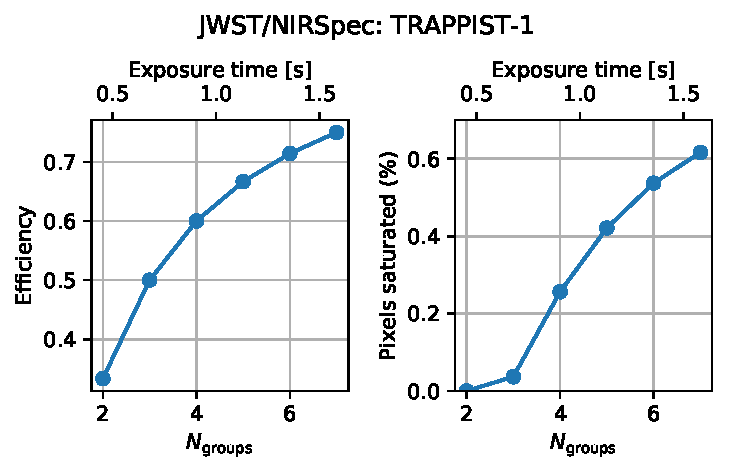
\includegraphics[scale=0.65]{libra/efficiency.pdf}
    \caption{Observing efficiency for different NIRSpec configurations using the SUB512 subarray on TRAPPIST-1 (J=11.354).}
    \label{fig:efficiency}
\end{figure}

\subsection{IRTF Spectral Templates}

We represent the host-star spectra with flux-calibrated infrared template spectra collected by \citet{Cushing2005} and \citet{Rayner2009} on the SpeX instrument on the NASA Infrared Telescope Facility (IRTF) \citep{Rayner2003}. 

\begin{table}
\centering
\begin{tabular}{lccl}
Target & $T_{\mathrm{eff}}$ & Spectral & IRTF\\
 & [K] & Type & Template \\ \hline\hline
Kepler-296 & 3526 & M2V & HD 95735 \\
TRAPPIST-1 & 2511 & M8V & Gl 752B\\
Kepler-62 & 4926 & K2V & HD 3765\\
\end{tabular}
\caption{Target stars for TTV observations with JWST, and NASA IRTF Spectral Library template stars that we use as their spectral analogs. \label{tab:temps}}
\end{table}

We can compute the number of photons received by JWST from the flux-calibrated IRTF spectra, $f_\lambda$, with units W m$^{-2}$ $\mu$m$^{-1}$. For a telescope with aperture area $A$, with spectroscopic resolution elements of width $\Delta \lambda$, and exposure time $\Delta t$, the flux measured within each resolution element is: 
\begin{equation}
f_\lambda = \frac{hc}{\lambda} \frac{N_{\mathrm{template}}}{\Delta t A \Delta \lambda}
\end{equation}
where $N_{\mathrm{template}}$ is the number of photons received from the template star. Solving for $N_{\mathrm{template}}$,
\begin{equation}
N_{\mathrm{template}} = \frac{\lambda}{hc} \Delta t A \Delta \lambda f_\lambda.
\end{equation}
The templates are observations of real stars with magnitude $J_{\mathrm{template}}$, and we are interested in the counts received from a source with magnitude $J_{\mathrm{target}}$, so the number of photons received from the target star $N_{\mathrm{target}}$ is
\begin{equation}
N_\mathrm{target} = N_\mathrm{template} 10^{\Delta J / 2.5}
\end{equation}
where $\Delta J=J_\mathrm{template} - J_\mathrm{target}$. The measured detector gain of the NIRSpec detectors is close to unity, so $N_\mathrm{target}$ describes the number of counts registered by the detector. 

\subsection{Starspots}

The spot covering fraction of TRAPPIST-1 is an area of rapidly evolving literature, at present \citep{Rackham2018, Morris2018c, Zhang2018, Wakeford2019}. The stellar photosphere contains several temperature components, possibly including both dark and bright regions. We adopt the hypothetical scenario presented in \citet{Morris2018c}, where there are a few bright (hot) spots. This model reproduces the apparent rotational variability in the \kepler band, and lack of corresponding variability in the \spitzer band. It is possible that in fact the star does not have bright spots and a rotation period of 3.3 d, in which case adopting the \citet{Morris2018c} model will produce the most conservative estimates in the uncertainties on the transit depths and times. We assume spots have the spectrum of the IRTF template K0V star HD 145675, and a surface distribution consistent with the spot positions and radii of \citet{Morris2018c}.

The spot distribution of Kepler-62 is also unconstrained by the available observations. Given its similarities to the Sun in rotation period and spectral type, we assume a spot distribution like the Sun's is appropriate for Kepler-62. Given its long apparent rotation period (36 days, \citealt{Borucki2013}), and the small total flux variations imparted by sunspots, we thus ignore the rotational modulation of spots on Kepler-62.

\subsubsection{Covering fraction lower limit: Flux deficit}

\begin{figure}
\centering
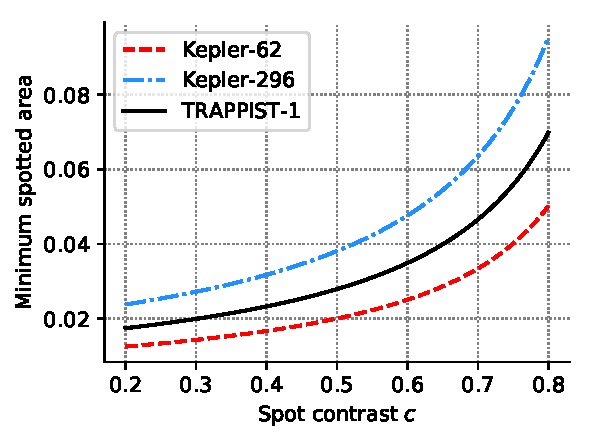
\includegraphics[scale=0.8]{libra/flux_deficits.pdf}
\caption{Approximate minimum spotted areas, approximated by the rotational modulation of each star in the \kepler or K2 light curves. }
\label{fig:deficit}
\end{figure}

We measure the minimum spotted area on each of the three stars using the flux deficit technique \citep[see e.g.][]{Morris2017a}. The minimum spotted area $f_S$ on the observer-facing hemisphere is 
\begin{equation}
f_S = (1 - \min(\mathcal{F})) (1 - c)
\end{equation}
where $\mathcal{F}$ is the set of observed fluxes normalized to the maximum flux in the light curve, and $c$ is the spot intensity contrast, such that spots with $c=0$ are perfectly dark, and spots with $c=1$ have the same intensity as the photosphere. $f_S$ is a lower bound on the spotted area, because in the limit of many spots distributed isotropically about the stellar surface, each spot that rotates out of view is replaced by another spot rotating into view, and the rotational modulation is small.

It is presently unclear if there are trends in spot contrast with stellar effective temperature \citep{Mancini2017}, so we consider the minimum spotted area for each star over a range of plausible spot contrasts in Figure~\ref{fig:deficit}. For comparison, the sunspot umbral contrast is $c\sim0.2$ and penumbral contrast is $c\sim0.8$ \citep{Solanki2003}. 

The flux deficit technique indicates that in the worst case -- where spots have $c=0.8$ -- each star must have at least 5\% of its observable hemisphere covered in stars. The flux deficit does not provide an upper limit on the spot covering fraction.

% \begin{figure}
% \centering
% 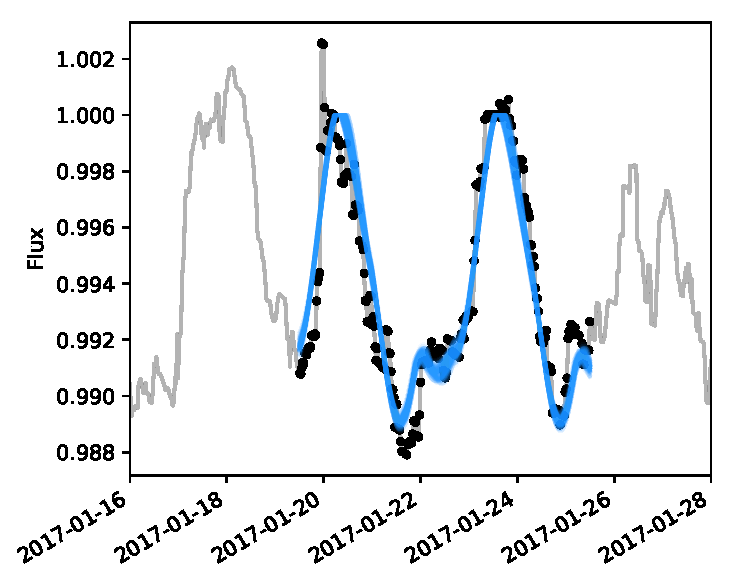
\includegraphics[scale=0.6]{libra/STSP_trappist1.pdf}
% \caption{Draws from the MCMC posterior samples of spot model fits (blue curves) to a two-rotation segment of the median-filtered TRAPPIST-1 K2 light curve (black circles), detrended with EVEREST. We include some of the surrounding light curve (gray) to demonstrate that the spots are evolving on the timescale of the rotation. Assuming there are three circular spots responsible for the rotation, the spots have characteristic sizes of $0.1 < R_\mathrm{spot}/R_\star < 0.2$, and contrasts of $0.4 < c < 0.6$.}
% \label{fig:stsp_trappist}
% \end{figure}


\begin{figure}
\centering
\includegraphics[scale=0.6]{libra/model_kepler296_darkspots.pdf}
\caption{Draws from the MCMC posterior samples of spot model fits (blue curves) to a two-rotation segment of the median-filtered Kepler-296  light curve (black circles). Assuming there are two circular spots responsible for the rotation, the spots have characteristic sizes of $0.1 < R_\mathrm{spot}/R_\star < 0.2$, and contrasts of $0.4 < c < 0.6$.}
\label{fig:stsp_k296}
\end{figure}

We compute the spotted area on the observable hemisphere of the star using the spot modulation algorithm in \citet{Morris2018b}. The spot model assumes circular spots and quadratic limb-darkening, and uses affine invariant MCMC to fit the light curve for spot radii, positions, and a global spot contrast parameter \citep{Foreman-Mackey2013}. Figure~\ref{fig:stsp_k296} shows a portion of the \kepler light curve of Kepler-296, and draws from the posterior distributions from the model fit. The corresponding maximum-likelihood spot temperature is $\sim 3300$ K, in good agreement with measured spot temperatures of similar M dwarfs \citep{Berdyugina2005}.

When we generate realizations of the star with its spots, we draw from the posterior distributions of the spot radii, contrasts and positions to place spots on the star. For Kepler-296, the long rotation period $P_\mathrm{rot} \sim 36$ d ensures that stellar rotational modulation does not cause significant variability on transit timescales.

% \subsubsection{Rotational modulation: TRAPPIST-1}

% \citet{Morris2018c, Zhang2018, Rackham2018}


% \begin{figure}
% \centering
% 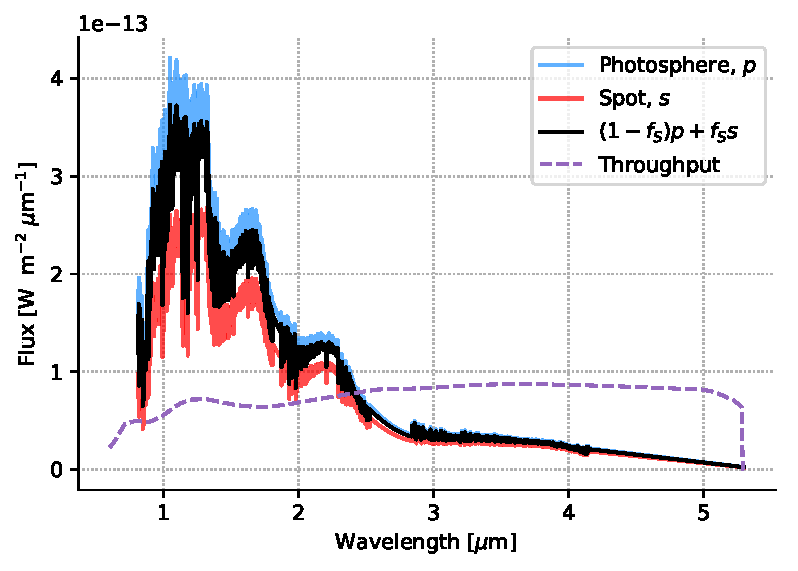
\includegraphics[scale=0.6]{libra/combo_atm.pdf}
% \caption{IRTF template spectrum of Gl 752B (blue), which we use as a proxy for TRAPPIST-1, with a scaled spectrum representing spots that are 200 K cooler (red). Assuming some spot covering fraction, e.g.~$f_S=0.4$ in this example, we approximate the spectra of spotted stars as linear combinations of spectra with the effective temperature of the photosphere, and the effective temperature of the spot (black).}
% \label{fig:combo}
% \end{figure}

We approximate the rotational modulation's effect on the stellar spectrum by modeling the stellar spectrum as a linear combination of spectra with the effective temperatures of the photosphere and spots. %The spot contrast posterior distributions from Section~\ref{sec:spotmodel} give approximate spot temperatures. 
We choose the nearest IRTF spectral template to the spot temperatures found for each star. 


\subsection{Flares}

The K2 EVEREST light curve of TRAPPIST-1 reveals several flare events \citep{luger2017everest}. We remove the stellar rotation and instrumental systematics by dividing the light curve by itself smoothed with a 31 cadence kernel median-filter. We fit the positive outliers with the \citet{Davenport2014} empirical flare model to solve for the typical flare peak flux and duration of 11 significant flares in the K2 light curve.%, see Figure~\ref{fig:flares}.
In simulated light curves, we sample flares from a Poisson process with a rate of 11 events per 78 days, and draw the peak-flux and duration parameters for each simulated flare from the fits to the observed K2 light curves. We assign the spectrum of a 10,000 K blackbody to each flare \citep{Kowalski2015}.

Kepler-62 had few significant flare events over the four years of \kepler observations, suggesting that the probability of a flare event occurring during a transit is negligible. 

Kepler-296 had $\sim 4$ significant flare events over the four years of \kepler observations, suggesting that the probability of a flare event occurring during a transit is negligible. 

\subsection{``Microvariability'' of TRAPPIST-1 at 4.5 $\mu$m}

An unidentified source of variability was observed in the \spitzer 4.5 $\mu$m light curve of TRAPPIST-1 of \citet{Delrez2018} after removing transits and flares. We detect a periodic signal in the autocorrelation function and the Lomb-Scargle periodogram of the light curve near 0.5 days. It is not clear whether or not the variability observed with \spitzer is due to stellar granulation or something else.

We model the quasi-periodic oscillations with Gaussian process regression using an exponential kernel \citep{Foreman-Mackey2017}. We include this variability observed at 4.5 $\mu$m in the light curve simulations, assuming there is no wavelength dependence. 

\begin{figure}
\centering
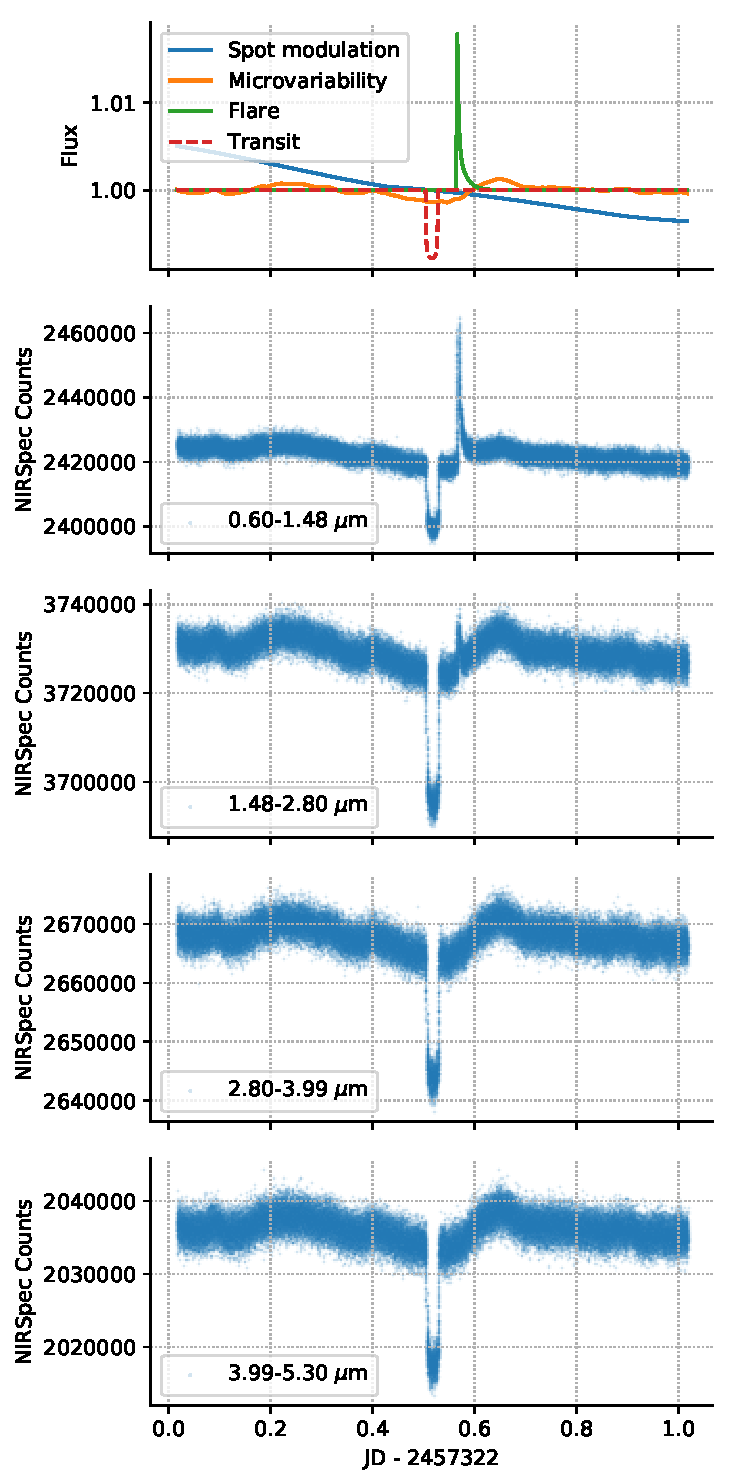
\includegraphics[scale=0.65]{libra/breakdown_long.pdf}
\caption{Simulated spectrophotometric observations of TRAPPIST-1 with JWST/NIRSpec, with $N_\mathrm{groups} = 6$, assuming the starspot distribution of \citet{Morris2018c}. The top-most panel shows the input components into the model, including the transit of TRAPPIST-1 b, rotational spot modulation, microvariability as observed in the Spitzer 4.5 $\mu$m band, a flare following the morphology of \citet{Davenport2014}.}
\label{fig:breakdownt1}
\end{figure}


\subsection{Scaling the \kepler-band variability of Kepler-62 and Kepler-296}

\begin{figure}
\centering
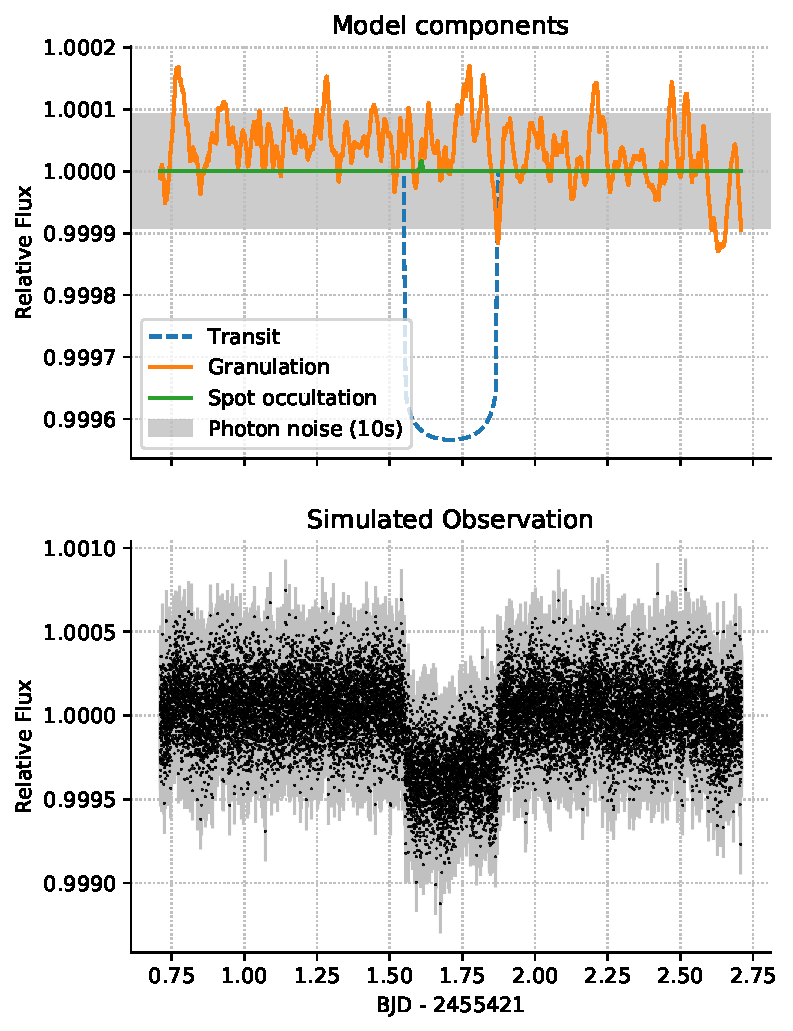
\includegraphics[scale=0.6]{libra/k62f_breakdown.pdf}
\caption{Scale of the microvariability (orange) compared to the photon noise (gray) and a band-integrated transit of Kepler-62 f (blue). We also show what a typical spot occultation might look like assuming Kepler-62 has a Sun-like spot distribution (green), which is significantly smaller than the microvariability and the photon noise.}
\label{fig:k62f}
\end{figure}

For Kepler-62 and Kepler-296, lacking empirical observations of the stellar variability in the near infrared, we must approximate the amplitude and functional form of the microvariability. We measure the microvariability directly by fitting a Gaussian process with an exponential kernel to the \kepler short-cadence light curve at short timescales. Then we must extrapolate the amplitude observed in the \kepler band to the NIRSpec bandpass. We assume that the microvariability is due to stellar granulation \citep{ludwig2002, tremblay2013, Trampedach2017}. In this section, we outline an approximation for estimating the amplitude of microvariability due to granulation in the NIRSpec band, given a measurement of the granulation amplitude in the \kepler band.

Ignoring limb-darkening, let's say a fraction $f_c \ll 1$ of the star is covered by the cool portion of granules with temperature $T_c$, while the remainder of the star we take as having a constant temperature, $T_s$.
Then, the flux from the star is given by:
\begin{equation}
F _ { \nu } = \Omega \left[ f _ { c } I _ { \nu } \left( T _ { c } \right) + \left( 1- f _ { c } \right) I _ { \nu } \left( T _ { s } \right) \right]
\end{equation}
we will assume the granule temperature is constant, so the only way that the flux can vary in the \kepler band is via a variation in $f_c$.  The specific intensity is $I_\nu(T)$ for an atmosphere at temperature $T$, while $\Omega$ is the solid angle of the star.

Then, integrating over the \kepler (subscript $K$) and JWST/NIRSpec Prism (subscript $P$) bands:
\begin{eqnarray}
\dot { N } _ { K } &=& \int d \nu \frac { F _ { \nu } } { h \nu } T _ { K ,\nu } \\ 
\dot { N } _ { P } &=& \int d \nu \frac { F _ { \nu } } { h \nu } T _ { N ,\nu }
\end{eqnarray}
where $T_{K,\nu}$ is the \kepler throughput at frequency $\nu$,
and $\dot{N}_K$ is the photon count rate (cm$^2$ s$^{-1}$).

When $F_\nu$ varies, this causes variation in $\dot{N}_K$ and
$\dot{N}_P$, but both of these just depend on $f_c$. Since the amplitude
of variation is small, we Taylor expand:
\begin{equation}
\dot { N } _ { K } = \dot { N } _ { K } | _ { f _ { 0} ,0} \left[ 1+ \left( f _ { c } - f _ { c ,0} \right) \frac { d \dot { N } _ { K } } { d f _ { c } } \frac { 1} { \dot { N } _ { K } | f _ { c ,0} } \right]
\end{equation}
Now,
\begin{multline}
\frac { d \dot { N } _ { K } } { d f _ { c } } \frac { 1} { \dot { N } _ { K } | _ { f _ { c } ,0} } =\\ \frac { \int d \nu \left[ I _ { \nu } \left( T _ { c } \right) - I _ { \nu } \left( T _ { s } \right) \right] \nu ^ { - 1} T _ { K ,\nu } } { \int d \nu \left[ f _ { c } I _ { \nu } \left( T _ { c } \right) + \left( 1- f _ { c } \right) I _ { \nu } \left( T _ { s } \right) \right] \nu ^ { - 1} T _ { K ,\nu } } \\
\approx \frac { \int d \nu  \left[ I _ { \nu } \left( T _ { c } \right) - I _ { \nu } \left( T _ { s } \right) \right]  \nu ^ { - 1} T _ { K ,\nu } } { \int d \nu I _ { \nu } \left( T _ { s } \right) \nu ^ { - 1} T_{K ,\nu} }
\end{multline}
where the approximation assumes $f_c \ll 1$. A similar relation holds for NIRSpec/Prism. Thus, the ratio of the fractional amplitude of
variation in NIRSpec/Prism to that in \kepler, $\alpha$, is given by:
\begin{multline}
\alpha \equiv \left( \frac { d \dot{N} } { d f _ { c } } \frac { 1} { \dot { N }_P | f _ { c ,0} } 
\right)  \left( \frac { d \dot{N} _ { K } } { d f _ { c } } \frac {1} { \dot{N} _ { K } | f _ { c ,0} } \right)^{-1} \approx\\
\frac { \int d \nu [I_\nu(T_c)-I_\nu(T_s)] \nu ^ { - 1} T _ { P ,\nu } } { \int d \nu [I_\nu(T_c)-I_\nu(T_s)] \nu ^ { - 1} T _ { K ,\nu } } \frac { \int d \nu I _ { \nu } \left( T _ { s } \right) \nu ^ { - 1} T _ { K ,\nu } } { \int d \nu I _ { \nu } \left( T _ { s } \right) \nu ^ { - 1} T_{P ,\nu}}
\end{multline}

\citet{Trampedach2013} estimates that for a star like Kepler-62, the intensity contrast due to granulation $ I_\mathrm{rms} / \left<I\right> = 0.12$ (see their ``simulation 33''), which implies $\alpha \approx 0.8$. For Kepler-296 with $I_\mathrm{rms}/\left<I\right> = 0.07$ (``simulation 36'') we find $\alpha \approx 0.85$.

% Granulation: \citet{Ludwig2002, Tremblay2013, Trampedach2017}

\subsection{Transits}

We inject \citet{Mandel2002} transits $\mathcal{T}(t)$ into the simulated spectrophotometry of TRAPPIST-1 assuming spots are unocculted by the planets,
\begin{equation}
\mathcal{F}_{\lambda}(t) = (\mathcal{T}(t) - f_S(t))F_{\lambda, \mathrm{photo}} +\\
f_S(t) F_{\lambda, \mathrm{spot}},
\end{equation}
where $f_S(t)$ is the spotted area as a function of time, $F_{\lambda, \mathrm{photo}}$ is the spectrum of the photosphere, and $F_{\lambda, \mathrm{spot}}$ is the spectrum of a starspot. 


Kepler-296 is a binary system with a faint companion M star, so we modify the above equation accordingly:
\begin{equation}
\mathcal{F}_{\lambda}(t) = \epsilon ( (\mathcal{T}(t) - f_S(t))F_{\lambda, \mathrm{photo, primary}} + f_S(t) F_{\lambda, \mathrm{spot}} ) + (1 - \epsilon) F_{\lambda, \mathrm{photo, secondary}},
\end{equation}
where $\epsilon = 0.785 \pm 0.012$ is the flux dilution factor \citep{Barclay2015}, and $F_{\lambda, \mathrm{photo, secondary}}$ is the spectrum of the secondary star. We assume that the amplitude of the secondary star's rotational variability is small compared to the primary star.

\subsection{Injected transmission spectra}

% Brett: the description here sort of depends on which atmosphere types you end up using. If you only use the CO2-dominated ones, I'll leave out mention of photochemistry. The O2/aqua planet atmospheres were generated using self-consistent photochemistry, another advantage worth mentioning here. Also, this is a draft for now and probably needs revision later... --Andrew

We generate transmission spectra by placing a wavelength-dependence on the simulated transit depth. We adopt high-resolution simulated transmission spectra from \citet{Lincowski2018}, which are generated using a line-by-line, multi-stream, multi-scattering radiative transfer model \citep[SMART;][]{Meadows1996} that has been validated for a wide variety of terrestrial atmospheres, including Earth \citep{Robinson2011}, Mars \citep{Tinetti2005}, and Venus \citep{Meadows1996,Arney2014}. The temperature profiles for the simulated spectra were generated by \citet{Lincowski2018} using a new 1D radiative-convective-equilibrium climate model, VPL~Climate \citep{Robinson2018,Lincowski2018}, which uses SMART as its core for radiative transfer, and has been validated for Earth, Mars, and Venus \citep{Robinson2018}. The simulated cloudy Venus-like atmospheres included the vertically-resolved radiative effects of aerosols.
To generate the climate states and spectra for the oxygen-dominated, post-runaway greenhouse atmospheres posited by \citet{Luger2015b}, \citet{Lincowski2018} coupled VPL~Climate to a terrestrial-based photochemistry model, to self-consistently include the effects of the M~dwarf host star spectrum on abundances of atmospheric trace gases, and hence spectral signatures that might be observed by JWST. 


% \begin{figure}
% \centering
% 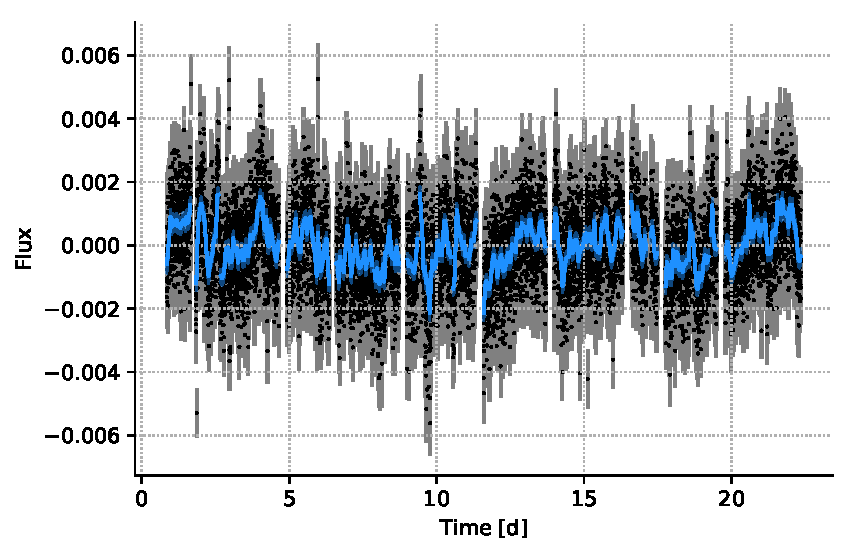
\includegraphics[scale=0.6]{libra/gp.pdf}
% 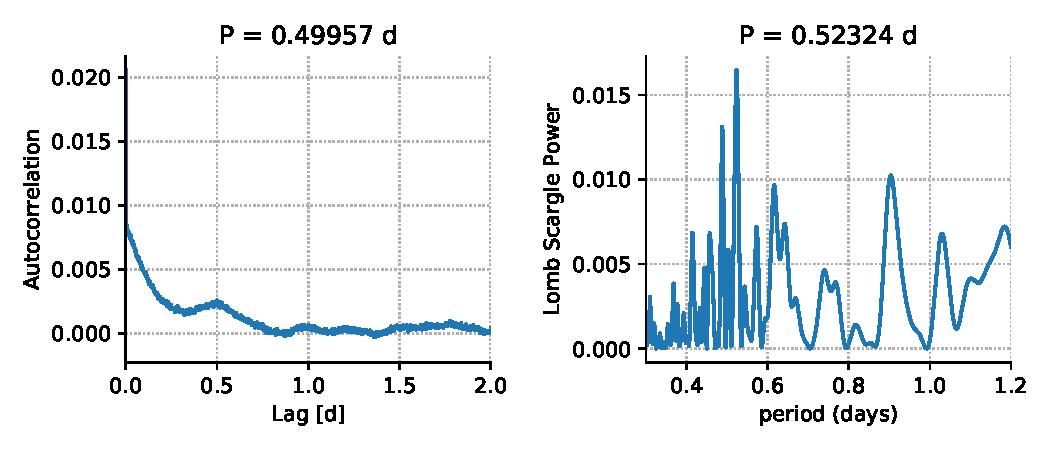
\includegraphics[scale=0.5]{libra/quasiperiodic.pdf}
% \caption{\textsl{Upper:} Spitzer 4.5 $\mu$m variability after removing flares and transits (black circles), and a Gaussian process regression modeled with a simple-harmonic oscillator kernel (blue curve). \textsl{Lower:} The autocorrelation function and Lomb-Scargle periodogram of the Spitzer 4.5 $\mu$m observations, both showing a peak near period 0.5 d.}
% \label{fig:gp}
% \end{figure}


% \begin{figure}
% \centering
% 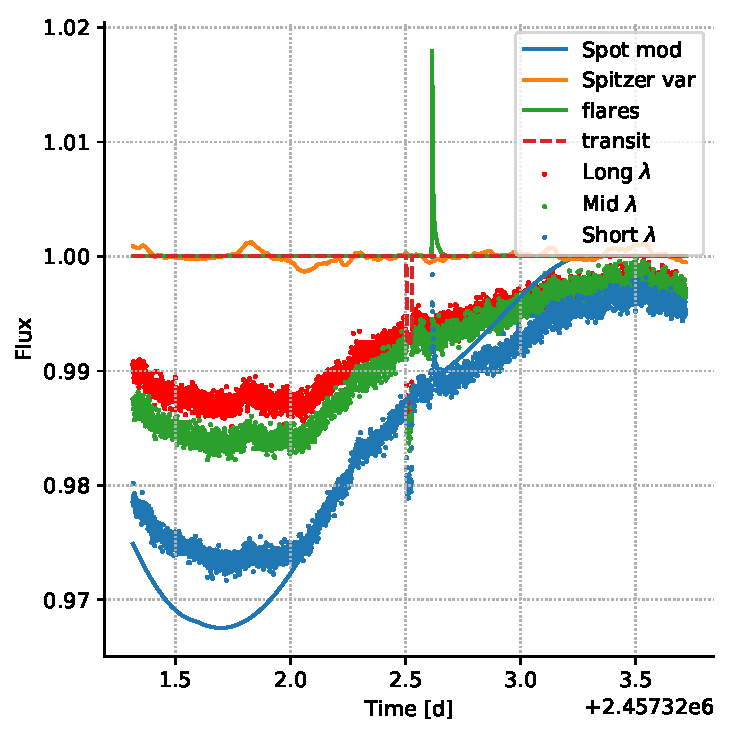
\includegraphics[scale=0.6]{libra/breakdown.pdf}
% \caption{Simulated transit observations of TRAPPIST-1 b, including the effects of spot modulation, stellar flares, and the unindentified 4.5 $\mu$m variability observed in the Spitzer data. The simulations produce a series of spectra in time --- here we bin the spectra into three bins, ``long, mid, short'', and plot the }
% \label{fig:breakdown}
% \end{figure}

\section{Analysis of synthetic observations}

\subsection{Gaussian-process regression}

% \begin{figure*}
% \centering
% 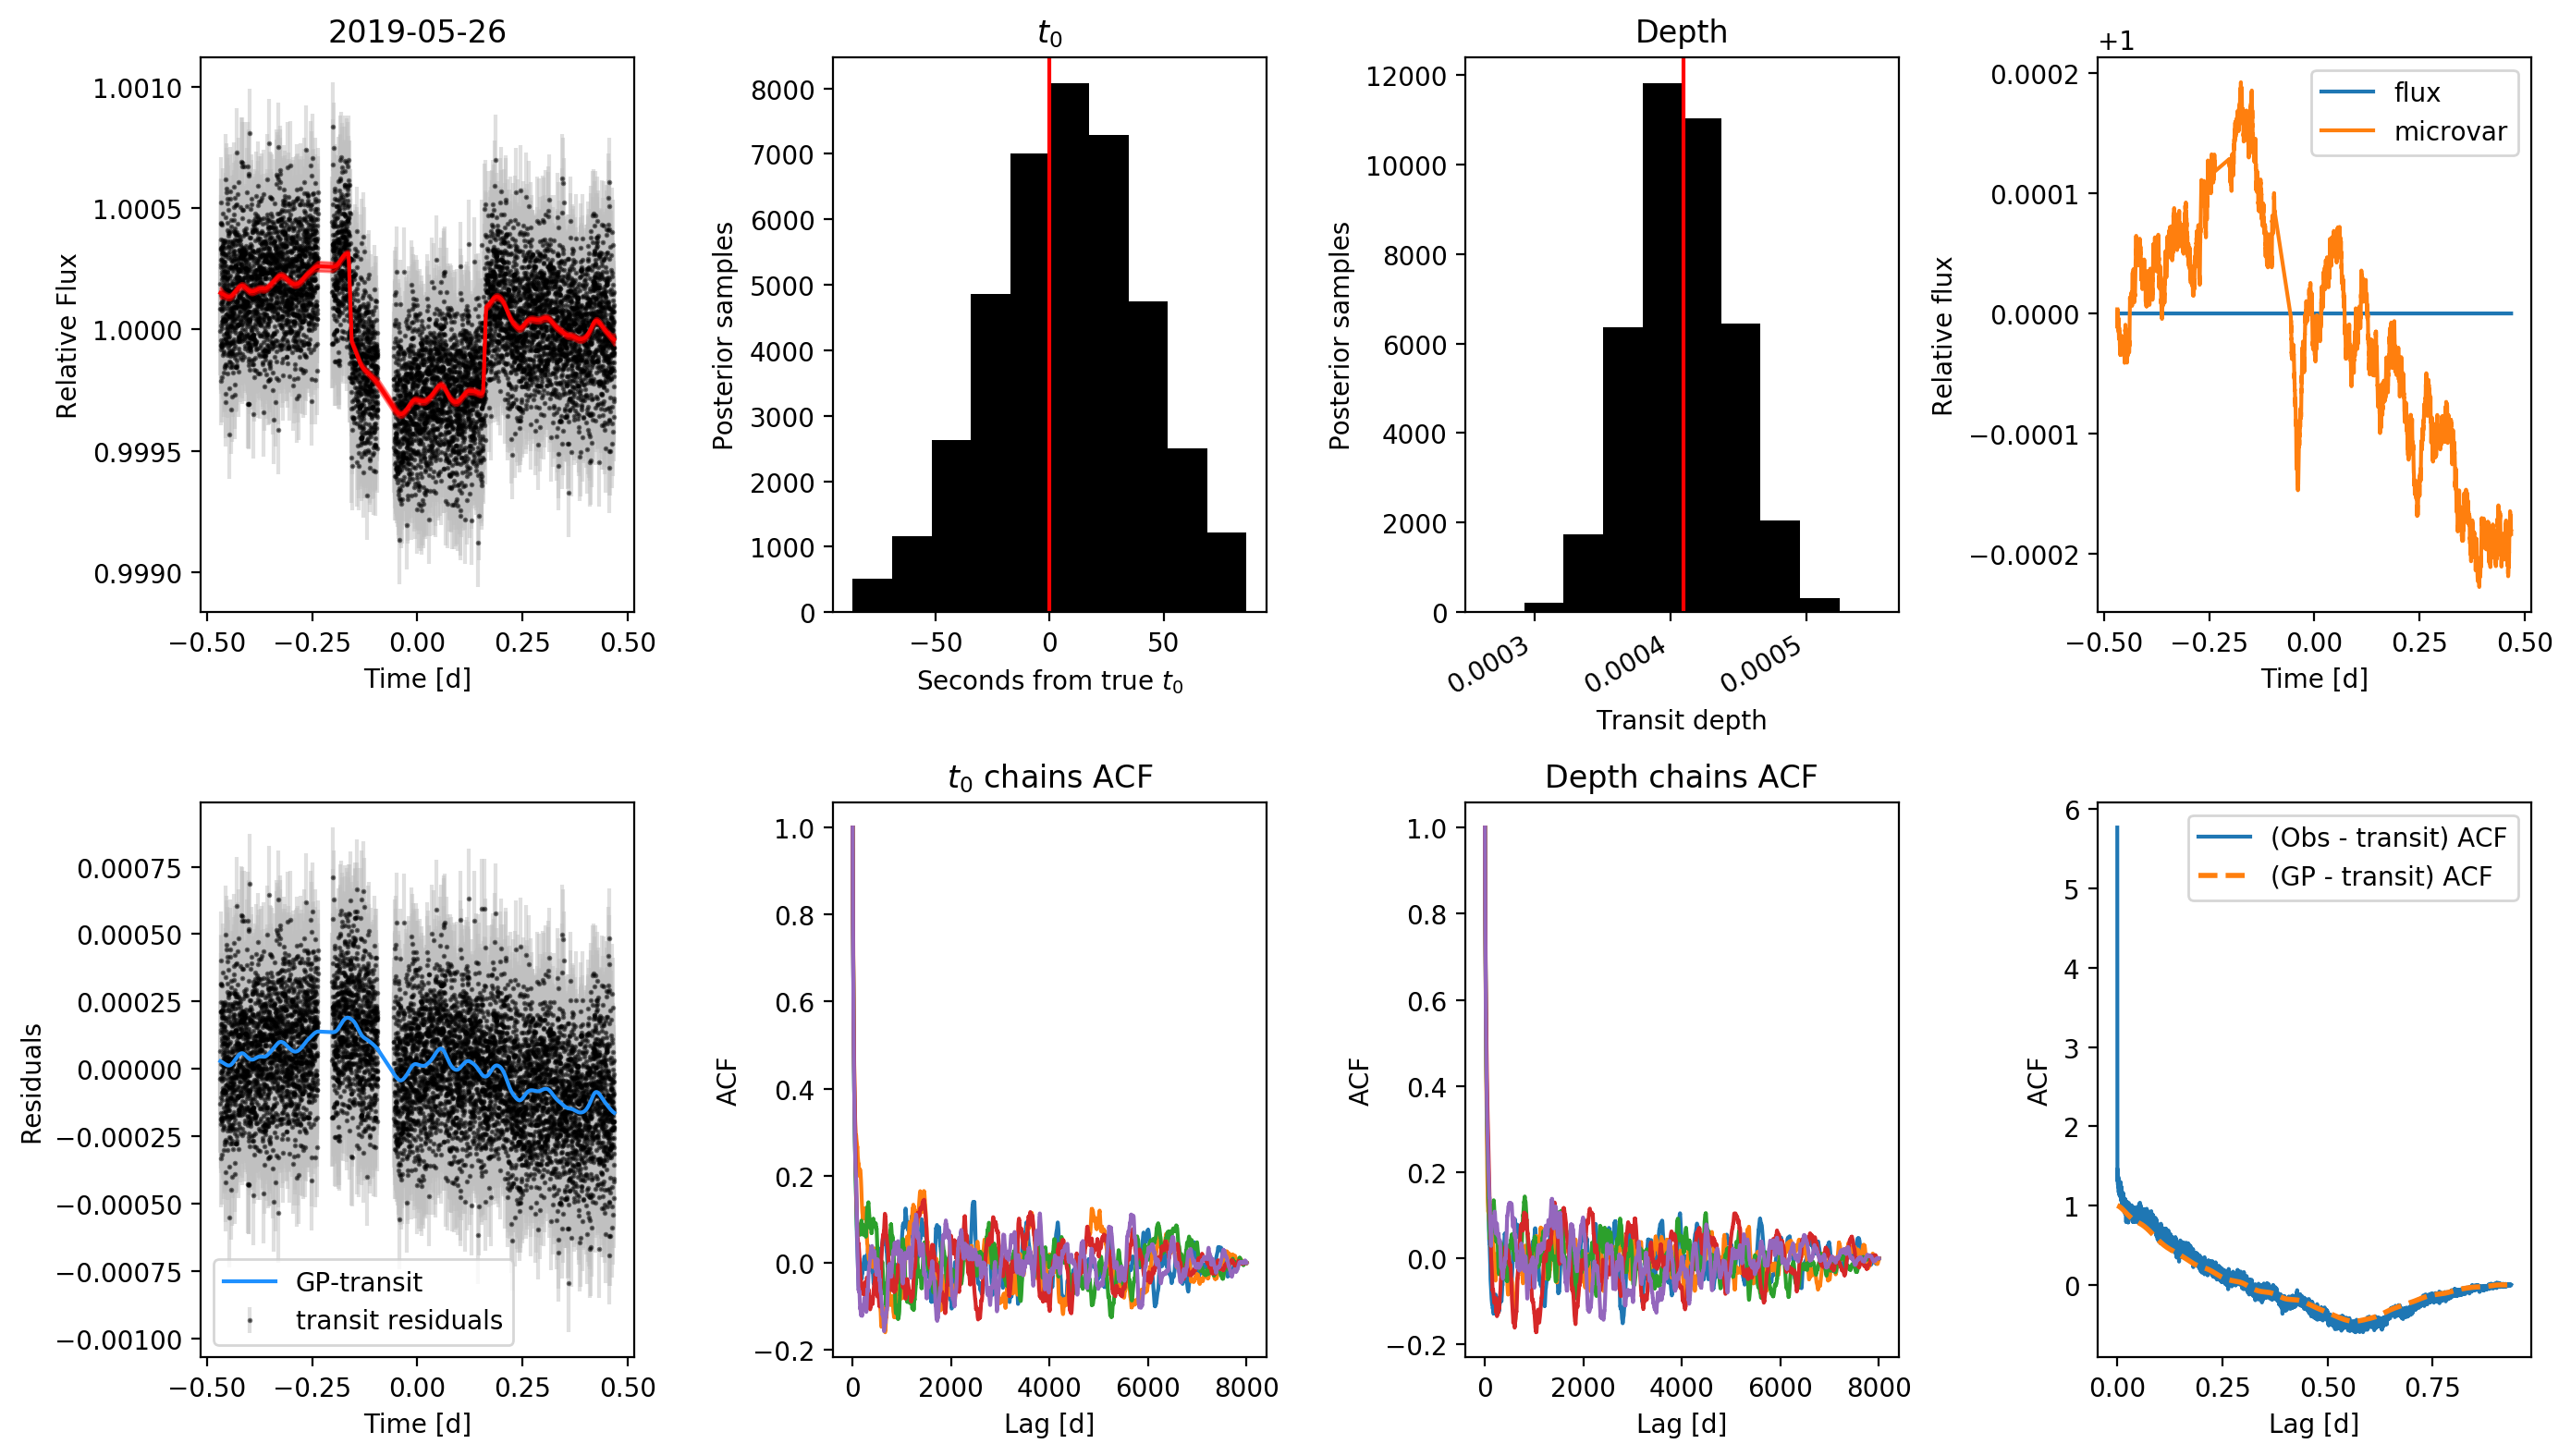
\includegraphics[scale=0.5]{libra/results_2458629_f.png}
% \caption{Fit to a simulated transit of Kepler-62 f. The left-most column shows the simulated transit photometry integrated over the NIRSpec Prism band (black circles), masked during transtis of other planets in the system (gaps), and the maximum-likelihood Gaussian process kernel convolved with the data (red curve in upper panel, blue in lower). The middle two columns show histograms and autocorrelation functions for posterior samples for the mid-transit time $t_0$ and transit depth. The upper-right panel shows the microvariability realization for this observation, and the static flux of the host-star (assuming small rotational modulation). The lower-right panel shows that the maximum-likelihood Gaussian process kernel is a good fit to the observations after removing the transit model.}
% \label{fig:fit}
% \end{figure*}

We fit each band-integrated transit with a \citet{Mandel2002} transit model. Ideally, we would like to detrend the transit observations against a set of observational basis vectors including: the spotted area of the star over time, and microvariability flux of the star over time, while modeling and removing any flares that occur during the observations. We anticipate lacking such supporting observations, and thus we model the correlated stellar noise with a Gaussian process (GP) \citep{Foreman-Mackey2017}. The flexible GP models allow us to sample accurate parameter uncertainties for the mid-transit times and depths without specifying the exact functional form of the variability.

We model the out-of-transit variability with a simple-harmonic oscillator (SHO) kernel, rather than the true input exponential kernel, since in practice we will not know the appropriate kernel function \textit{a priori}. We're likely to use a kernel like the SHO kernel because SHO kernels have desirable properties for smoothly varying observations of stellar variability -- they are periodic but damped, with small but finite power at high frequencies.

\subsection{Transit Timing Precision}

\subsubsection{TRAPPIST-1}

% Transit timing variations of the TRAPPIST-1 system have been reported in \citet{Grimm2018}. The authors show that it is necessary to simultaneously fit the masses and orbital parameters of all planets, as there are many degeneracies between fitting parameters. 

We now compute the mass uncertainties on the planets TRAPPIST-1 b and c. First, we compute the expected transit times during the JWST mission, conditioned on the observed transits reported in \citet{Grimm2018}. We use \texttt{TTVFast} to solve for the masses, orbital periods, eccentricities, and mean anomalies and their uncertainties for planets e and f simultaneously using MCMC. 

We keep the eccentricities of planets b and c fixed at zero, as analysis by \citet{Luger2017} showed that eccentricities of b and c are tidally damped below $e < 0.01$. We also put Gaussian priors on the masses of each planet with the maximum-likelihood values and standard deviations reported by \citet{Grimm2018}.

By conditioning our TTV fits on the transits of \citet{Grimm2018}, we recover masses for b and c of $M_b = 1.12 \pm 0.17 M_\oplus$ and $M_c = 1.10 \pm 0.15 M_\oplus$ (consistent with the mass prior). Next we project 10 transit times of each planet (consistent with the proposed transmission spectroscopy observations proposed in Section~\ref{sec:transspec}), and recover the masses with \texttt{TTVFast}. The additional ten transits of each planet do little to add to the mass constraints -- the posterior mass distributions for each planet are consistent with the prior from \citet{Grimm2018}, indicating that transit timing variations of planets b and c from JWST are unlikely to yield much more information on the planet masses.  %[How much of this mass constraint results from the conditioning?  Is this typical of other draws from the prior conditioned on the current data? -EA] 

\subsubsection{Kepler-62}

We now compute the mass uncertainties on the planets Kepler-62 e and f using transit timing variations observed in our simulated transits. First, we must compute the expected transit times of planets e and f during the JWST mission, conditioned on the observed transits of each planet with \kepler and the Hubble Space Telescope (HST, cite Burke). We use \texttt{TTVFast} to solve for the masses, orbital periods, eccentricities, and mean anomalies and their uncertainties for planets e and f simultaneously using MCMC. 

Priors are critical to attaining convergence in our \texttt{TTVFast} fits. We place a uniform prior on eccentricity $e < 0.32$ consistent with dynamical modeling by \citet{Shields2016}. We compute the most-likely masses for Kepler-62 e and f using \citet{Chen2017} \texttt{forecaster} tool, which predicts masses for a given radius, assuming the planetary radii from \citet{Berger2018}, yielding probabilistic masses $M_e = 4.45^{+3.18}_{-1.68} M_\oplus$ and $M_f = 3.26^{+2.10}_{-1.15} M_\oplus$ -- and place Gaussian priors on the mass of each planet, centered on the maximum-likelihood mass and taking the maximum of the two-sided errorbars for the standard deviation. We also enforce the Hill stability criterion of \citet{Gladman1993} at each step in the MCMC chains. 

Next we select the maximum-likelihood iteration of the MCMC chains to predict future transit times of the Kepler-62 system, shown in Figure~\ref{fig:ttv_predicted}. One interesting feature of the maximum-likelihood solution are occasional 20 minute excursions from the expected midtransit time of a system without TTVs, which would be excellent times for observing the system to verify or falsify the maximum-likelihood combination of masses and orbital parameters. 

Typical timing precisions for the simulated transits of Kepler-62 e and f are 25 and 41 seconds, respectively. It is critical that we observe Kepler-62 e and f for as long as possible, and not just during ingress and egress -- the portions of the light curve which constrain the midtransit time. The stellar variability is similar in amplitude and timescale to the ingress and egress, and so integrating over a long time baseline is necessary to properly measure and marginalize over the stellar variability with Gaussian process regression.

We next test an optimistic scenario, assuming that JWST observes every transit of Kepler-62 e and f during its nominal five year mission (this isn't actually possible since the target is not in the continuous viewing zone). This amounts to 15 transits of e and 6 transits of f. The mass posteriors for this ``all-in'' every-transit campaign are shown in Figure~\ref{fig:mass_posteriors}. We can measure the masses of each terrestrial planet accurately and to 10\% precision. We note that this remarkable feat is not possible with modern radial velocity techniques -- the only way to measure habitable terrestrial planet masses for a Sun-like star such as Kepler-62 is with this type of resource-intensive photometric TTV campaign.

If we instead calculate the mass precisions from TTV measurements accounting for the finite observability of Kepler-62 from JWST using the most recent version of APT, we find that there will be seven observable transits of planet e and four transits of planet f. Typical mass precisions retrieved from these transits have 10\% precision for planet f, and 20\% precision for planet e.  

\begin{figure*}
    \centering
    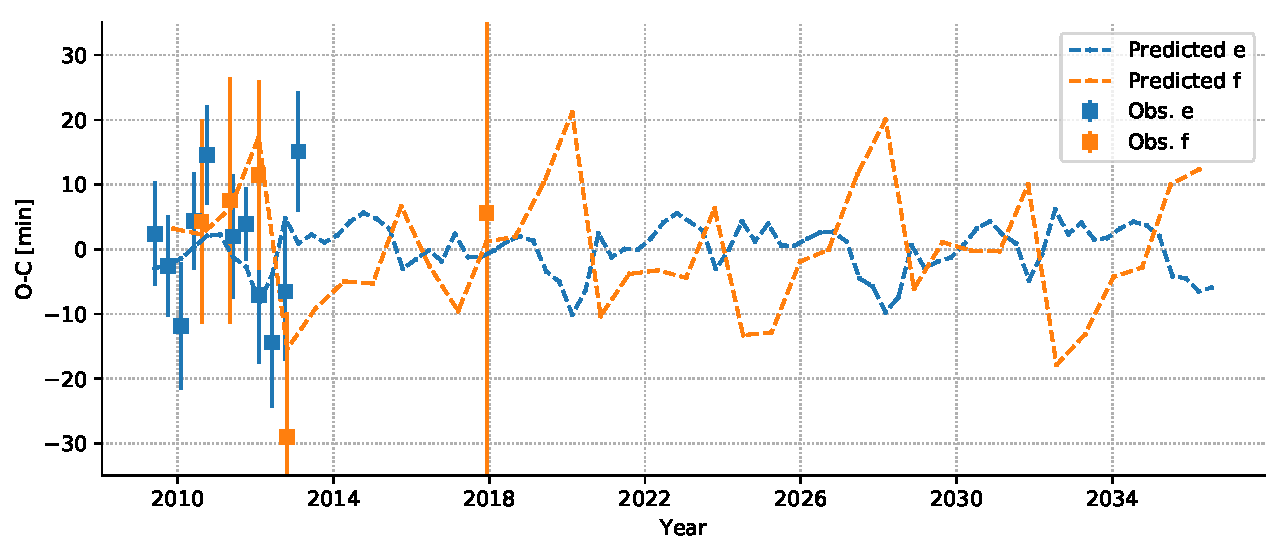
\includegraphics[width=\textwidth]{libra/ttvs_predicted.pdf}
    \caption{Predicted transit times using \texttt{TTVFast} to predict the transit timing variations of Kepler-62 e and f. }
    \label{fig:ttv_predicted}
\end{figure*}

\begin{figure}
    \centering
    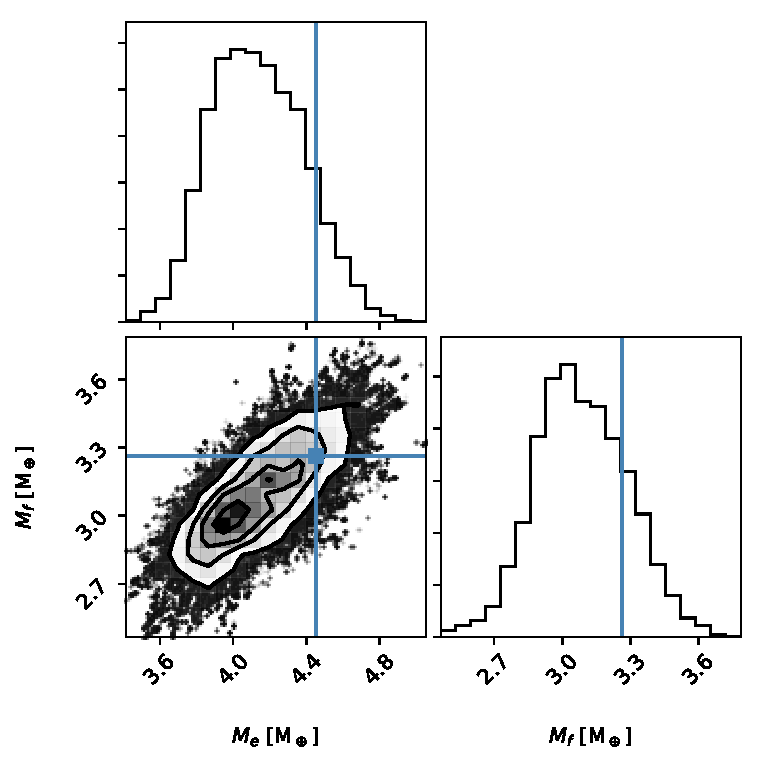
\includegraphics[scale=0.6]{libra/masses_kitchen_sink.pdf}
    \caption{Posterior distributions for the masses of Kepler-62 e and f, assuming JWST observes every transit of each planet over its five year nominal mission. We achieve mass precisions of order 10\% for both terrestrial planets. The input parameters to the simulated observations are shown in blue, confirming that the TTVs recover the correct masses within 1$\sigma$.}
    \label{fig:mass_posteriors}
\end{figure}

\begin{figure}
\centering
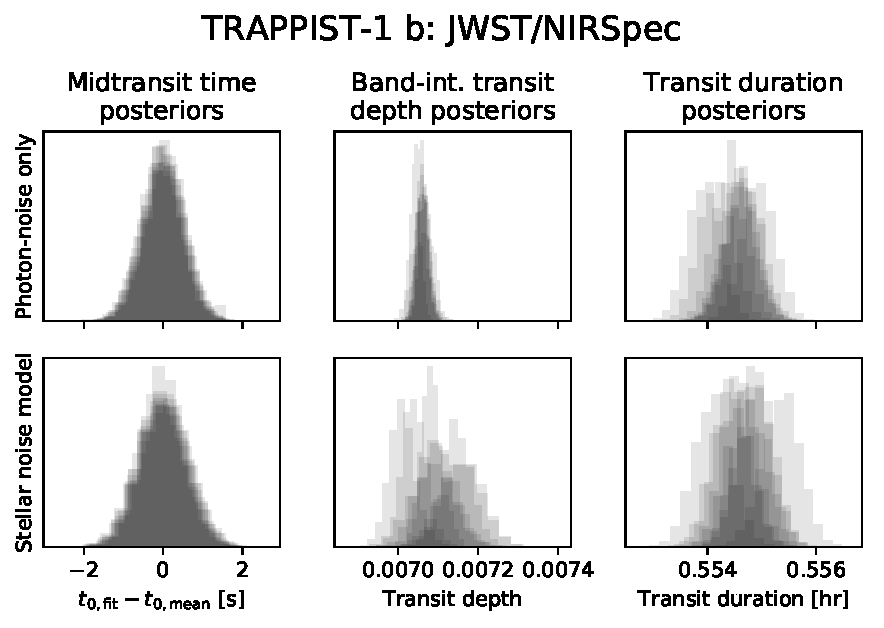
\includegraphics[scale=0.55]{libra/photon_vs_stellar_noise_bandint_t1.pdf}
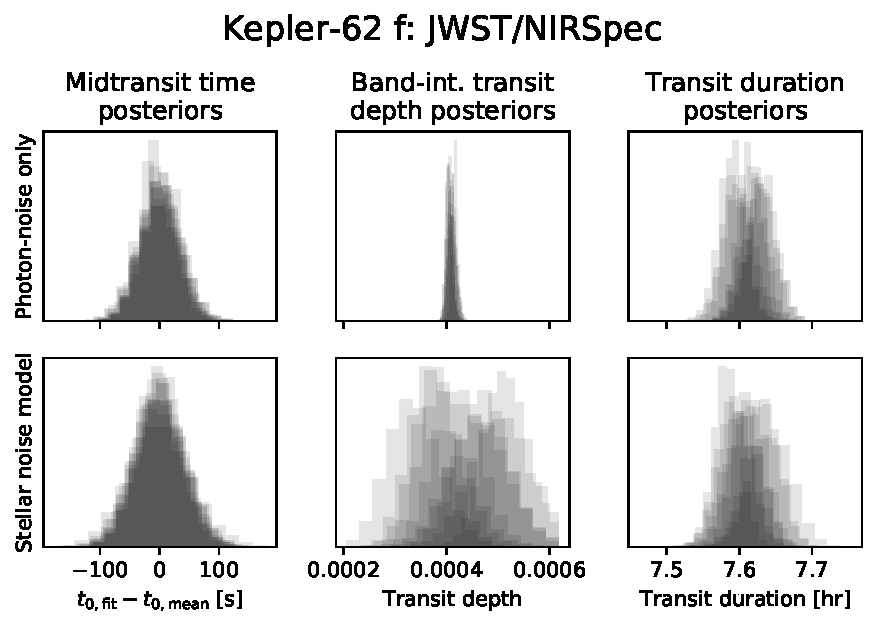
\includegraphics[scale=0.55]{libra/photon_vs_stellar_noise_bandint_k62.pdf}
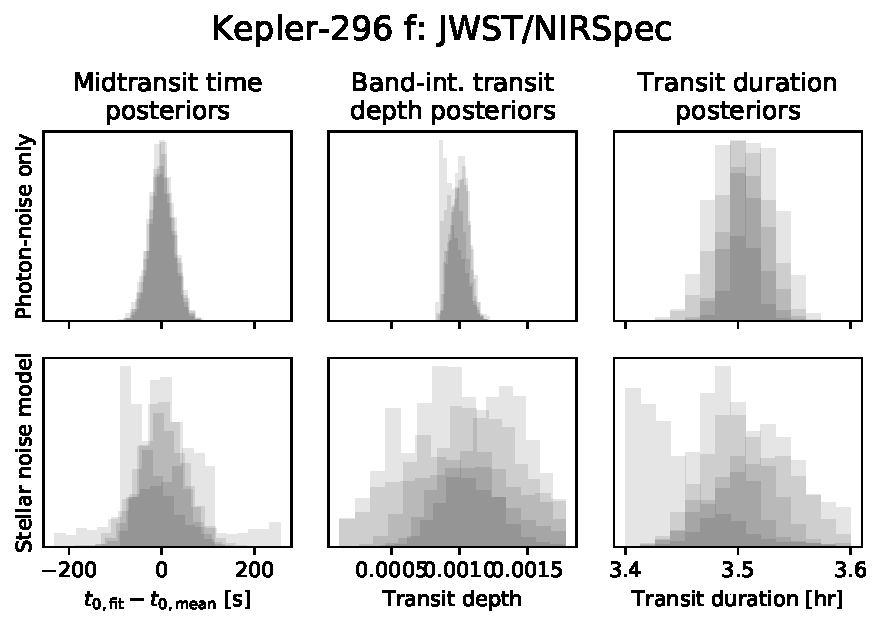
\includegraphics[scale=0.55]{libra/photon_vs_stellar_noise_bandint_k296.pdf}
\caption{Posterior distributions on the mid-transit times and depths given a photon-noise only model, compared with the full stellar activity model. The stellar activity model does little to change the uncertainty on the transit times
but significantly increases the uncertainty on the absolute, band-integrated transit depth for Kepler-62, while the uncertainties in all parameters increase for Kepler-296.}
\label{fig:photon_noise}
\end{figure}

\subsection{Bulk Density Precision}

Taking the realistic mass precisions from the previous section accounting for the finite observability of Kepler-62 from JWST, we now estimate the bulk density precision feasible with NIRSpec/Prism given the uncertainties on $R_p/R_\star$ and $M_p$ for Kepler-62 e and f. Figure~\ref{fig:bulkdensity} shows the positions and uncertainties for planets e and f on the mass-radius diagram. The black circles represent the input radii, and masses which were predicted by \texttt{forecaster} and recovered by \texttt{TTVFast} (see previous section). Overplotted are curves for the mass-radius relations for solid exoplanets from \citet{Seager2007}. In this analysis, we have assumed that the mass and radius of the host star are known with great precision, and the uncertainty in the exoplanet radii and masses are dominated by uncertainties in the transit timing analysis and transit depth. In reality, the mass and radius of Kepler-62 is known to $\sim3\%$, so there will in fact be noticeable correlations between the mass and radius posterior solutions in Figure~\ref{fig:bulkdensity}. 

%[The precisions are such that it's likely that the dominant uncertainty on
%the masses and radii of the planets will be the mass and radius of the star, since it is only the ratio of the radii which is measured from the transit depth, and the ratio
%of the masses which is measured from TTVs.  However, the stellar density can be constrained from the duration-period relation of the five planets (Seager \& Mallen-Ornelas 2002).  Thus, I would expect the posterior distribution of the planetary mass-radius diagram to be {\it highly} correlated - this can be seen in the Grimm et al. 
%paper on Trappist-1, one of my main contributions to the paper.  -EA]


\begin{figure}
\centering
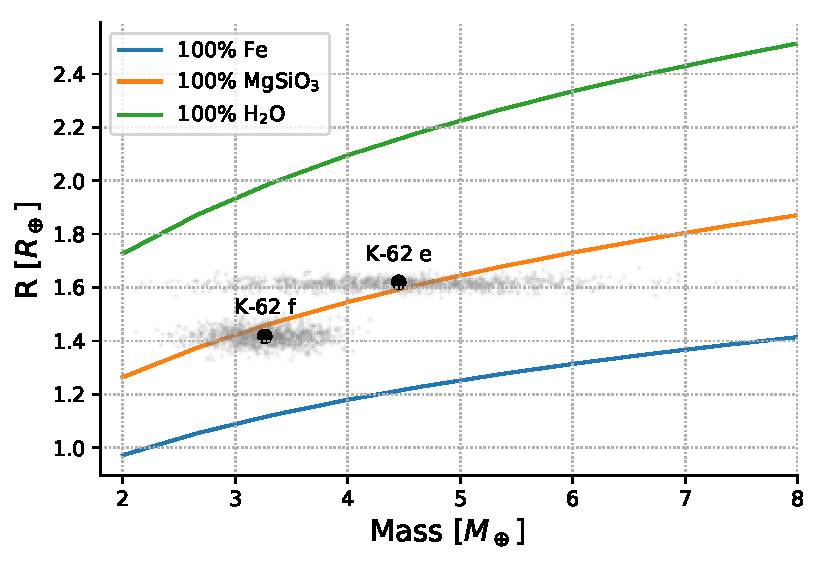
\includegraphics[scale=0.6]{libra/bulk_densities.pdf}
\caption{Mass/radius measurements attainable with a 5 year campaign for Kepler-62 e and f, with seven and four transits respectively, given the transit timing and planet radius precision predicted by our model. Black circles are the input masses and radii, the cloud surrounding them are the recovered posterior distributions in mass and radius. The curves show mass-radius relationships for solid exoplanets by \citet{Seager2007}. }
\label{fig:bulkdensity}
\end{figure}

\subsection{Transmission spectroscopy} \label{sec:transspec}

We measure transmission spectra by: (1) fitting the band-integrated light curve with a Gaussian process with an SHO kernel, masking out interloping transits of other planets, and (2) linearizing the combined Gaussian process and transit model, and fitting only for the transit depth as a function of wavelength at the native instrument resolution. This has the advantage of being computationally efficient, as the linear model is trivial to optimize, while avoiding any binning of the spectrum, which contains spectroscopic information at each wavelength.

\begin{figure*}
    \centering
    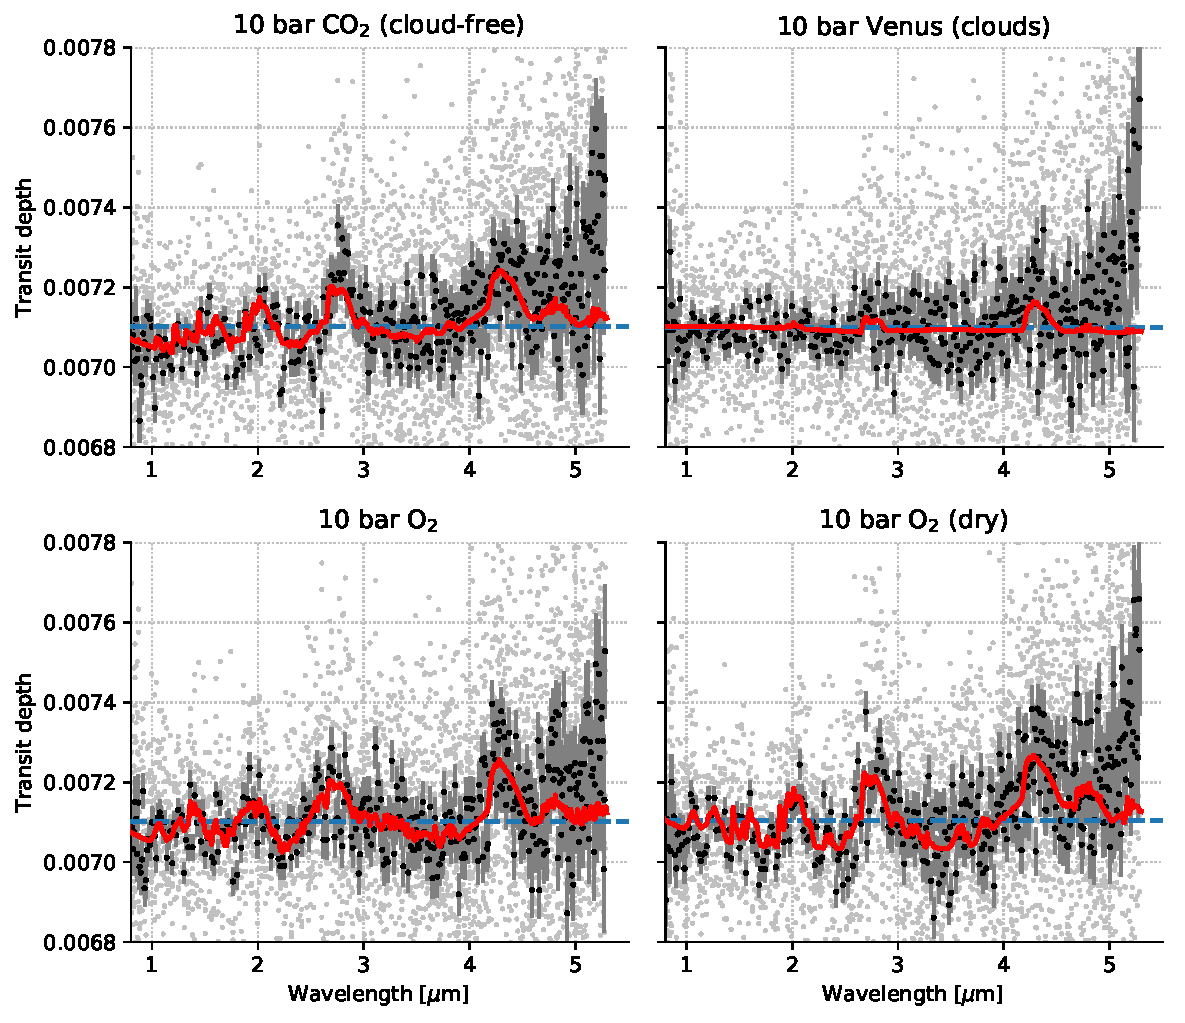
\includegraphics[scale=0.8]{libra/smart.pdf}
    \caption{Simulated JWST/NIRSpec Prism transmission spectra of TRAPPIST-1 b with 10 transits. The red curve shows the input model spectrum, the gray points show the unbinned transmission spectrum of TRAPPIST-1 b at the native instrument resolution. The black points show the binned spectrum of TRAPPIST-1 b.}
    \label{fig:my_label}
\end{figure*}

\subsubsection{Validation against PandExo}

\begin{figure}
\centering
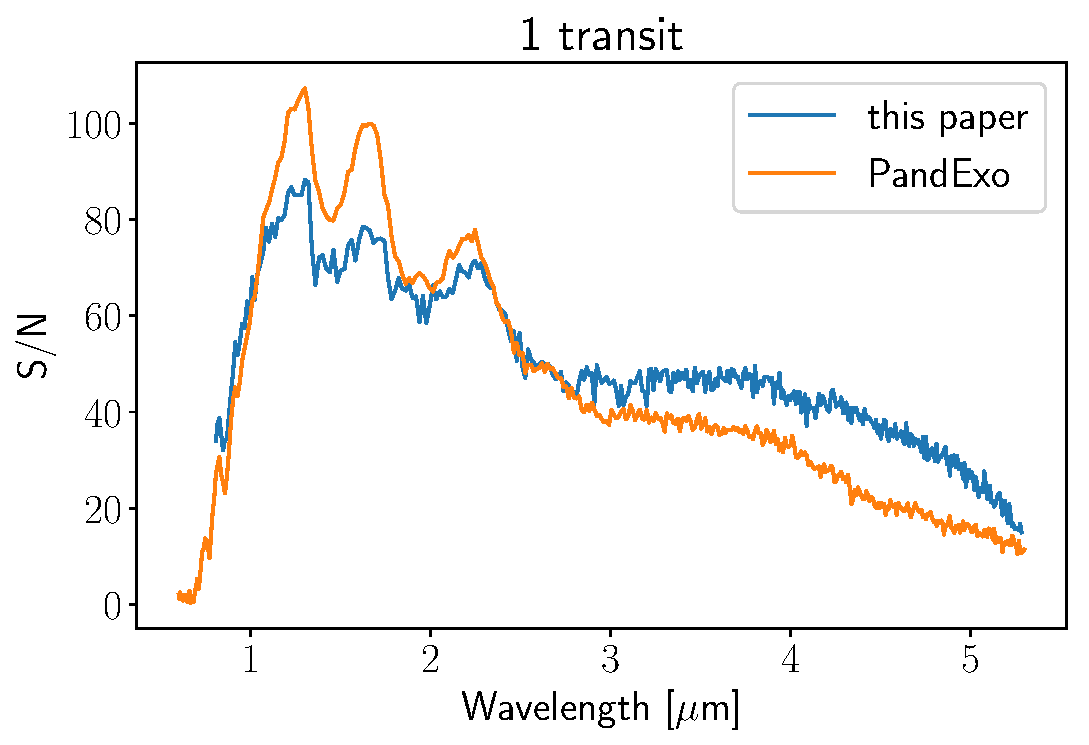
\includegraphics[width=0.47\textwidth]{libra/pandexo_libra_compare.pdf}
\caption{Signal-to-noise ratio on the transit depth for one transit of TRAPPIST-1 b with the JWST/NIRSpec Prism comparing \texttt{PandExo} (orange line) and the model developed in this paper (blue line).}
\label{fig:pandexo_snr}
\end{figure}

We compare our stellar variability noise model to the open-source and publicly available PandExo JWST noise model \citep{Batalha2017}. PandExo leverages the STScI's pixel-based signal-to-noise calculator, Pandeia \citep{Pontoppidan2016}, which forms the backbone of the official JWST exposure time calculator (ETC). We refer the reader to \citet{Batalha2017} and \citet{Pontoppidan2016} for a thorough description of PandExo and Pandeia, respectively. Briefly, for each calculation Pandeia simulates a spectral data cube at the pixel level which accounts for background noise, the point-spread-functions, instrument specific throughput and optical paths, pixel saturation levels, ramp noise, correlated read noise, flat field errors, and data extraction. Notably, it does not account to any time-dependent noise sources such as spacecraft drift and jitter or stellar variability. PandExo builds upon Pandeia to calculate transmission spectra of transiting exoplanets by considering in- and out- of transit wavelength dependent fluxes. PandExo does not simulate time-series spectro-photometry, but rather assumes a homogeneous stellar disk such that all in-transit time is equally viable observing time. This neglects the effects of stellar limb darkening and heterogeneous photospheres. 

Figure \ref{fig:pandexo_snr} compares the model we developed in the paper with PandExo for a single transit of TRAPPIST-1 b with the JWST/NIRSpec Prism. For this test, we assume that TRAPPIST-1 b possesses a CO$_2$ dominated cloud-free atmosphere \citep{Lincowski2018}. Both model simulations use the NIRSpec Prism with the SUB512 subarray with 6 groups per integration. The number of groups per integration results in 50 saturated pixels at the end of a ramp, however this allows for an observational efficiency of 71.4\%, compared to 33.3\% with no saturation when only 2 groups per integration are used. We find good agreement between our model and PandExo, with subtle and interesting deviations. Between $1-2.5$ $\mu$m, near the peak of the stellar SED, our model predicts lower S/N transmission spectra than PandExo by up to ${\sim} 25\%$. Beyond 2.5 $\mu$m our model predicts higher S/N than PandExo by ${\sim} 50\%$. We can reconcile these differences by considering that stellar photon noise dominates the transmission spectrum noise budget, so that when we account for the realistic time-dependence of the stellar spectrum we get less optimistic and more realistic noise estimates. % At longer wavelengths, the stellar SED decreases as a function of wavelength while the JWST background noise increases, (also stellar variability amplitude / spot contrast are lower) which makes PandExo more conservative.
Thus we conclude that the transmission spectrum S/N estimates of our simulated observations are consistent with PandExo.

\section{Discussion}

\subsection{Are the innermost planets of TRAPPIST-1 the best possible NIRSpec targets?}

Given that the JWST budget is approaching \$10 billion and the mission has a nominal lifetime of 5 years, the cost of observations to the taxpayer is roughly \$63 per second. With that price tag, robust justification must be made to invest in the long observing programs required to characterize exoplanets, and target lists must be carefully culled. 

Of the three targets we discuss in this paper, we note that TRAPPIST-1 b, c and d are perhaps \textit{the most optimal targets possible for characterization with JWST/NIRSpec} from several perspectives. Any target brighter than TRAPPIST-1 would either saturate the detector significantly for medium-duration exposures, or require very short exposures -- incurring a steep penalty in the observing efficiency. To date, there are no known exoplanet host stars smaller than TRAPPIST-1, maximizing the available transit depths for rocky planets. To the best of our knowledge, both planets b and c are probably rocky \citep{Weiss2014,Marcy2014,Rogers2015,Fulton2017}. The short orbital periods of the planets also ensure that each transit is short (about $\sim 80$ minutes) compared with transits of habitable zone planets orbiting Sun-like stars ($\sim 7.5$ hours). It would seem, by nearly every metric, it will be difficult to find terrestrial planets more amenable to follow-up with JWST/NIRSpec than TRAPPIST-1 b, c and d. 

It is presently unknown if TRAPPIST-1 b, c and d have atmospheres. If they have clear skies, we should be able to detect molecular absorption features with 10 transits or less. If they are cloudy or have no atmospheres, we will converge on flat transmission spectra by 10 transits. To distinguish between a Venus-like, cloudy planet and a rocky world with no atmosphere, additional instruments and observing techniques will be necessary -- planet-planet occultations, for example, are especially promising in this area \citep{Luger2017b}. 

Should we be fortunate enough to observe clear skies on TRAPPIST-1 b/c/d and the molecular absorption features have high enough S/N to discriminate between the different climate outcomes of \citet{Lincowski2018}, we may be able to say something about the atmospheric composition of a rocky exoplanet for the first time.

\section{Conclusions}

\begin{enumerate}
    \item JWST/NIRSpec is a high-throughput instrument with great potential to study exoplanets in the BOTS mode, provided it can be allowed to saturate for the brightest targets
    \item With transit timing variations, we are unlikely to better constrain the masses of TRAPPIST-1 b or c; though we can measure the masses of Kepler-62 e and f to 20 and 10\% respectively
    \item With the band-integrated transit depths and masses from TTVs, we can measure the bulk density of Kepler-62 e and f to 20\%
    \item Transmission spectroscopy of TRAPPIST-1 b and c may distinguish between the climate scenarios in \citet{Lincowski2018} with as little as 10 transits
    \item The innermost TRAPPIST-1 planets may be the most optimal observing targets for JWST/NIRSpec BOTS mode.
\end{enumerate}

%\acknowledgments
%
%We gratefully acknowledge support from NSF grant AST-1312453 and the NASA Astrobiology Institute under solicitation NNH12ZDA002C and Cooperative Agreement Number NNA13AA93A. A.P.L. acknowledges support from NASA Headquarters under the NASA Earth and Space Science Fellowship Program -- Grant 80NSSC17K0468. This research has made use of NASA's Astrophysics Data System.
%
%\facility{JWST/NIRSpec, IRTF/SpEX, \spitzer, \kepler}
%
%\software{\texttt{ipython} \citep{ipython}, \texttt{numpy} \citep{VanDerWalt2011}, \texttt{scipy} \citep{scipy},  \texttt{matplotlib} \citep{matplotlib}, \texttt{astropy} \citep{Astropy2013, Astropy2018}, \texttt{batman} \citep{Kreidberg2015} \texttt{celerite} \citep{Foreman-Mackey2017}, \texttt{gatspy} \citep{VanderPlas2016}, \texttt{emcee} \citep{Foreman-Mackey2013}, \texttt{forecaster} \citep{Chen2017}, \texttt{TTVFast}, \citep{Deck2014}}
%
%\bibliography{bibliography.bib}
%
%\appendix
%
%\section{Flares}
%
%\begin{figure*}
%\centering
%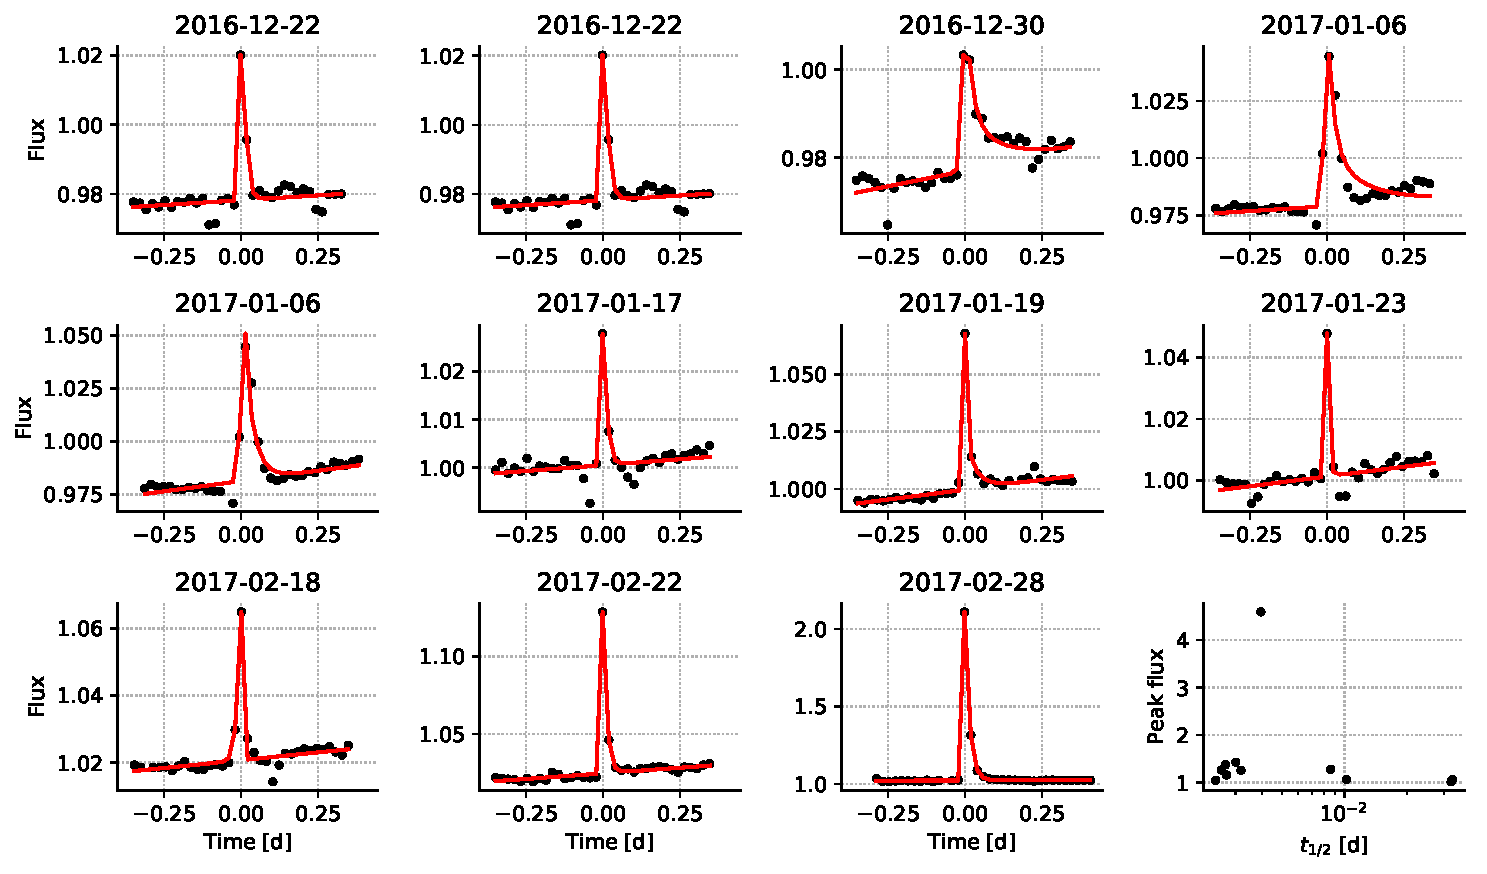
\includegraphics[scale=0.7]{libra/trappist1_flares.pdf}
%\caption{TRAPPSIT-1 flares observed with K2 via the EVEREST light curve from \citet{Luger2017}, fit with the empirical flare model from \citet{Davenport2014}. We inject flares into our simulated observations with  timescales and peak-fluxes drawn from these real flares.}
%\label{fig:flares}
%\end{figure*}


%\end{document}

